\section{Potential energy and equilibria}
	\setwrappadding
	\begin{wrapfigure}[15]{r}{0.5\textwidth}
		\centering
		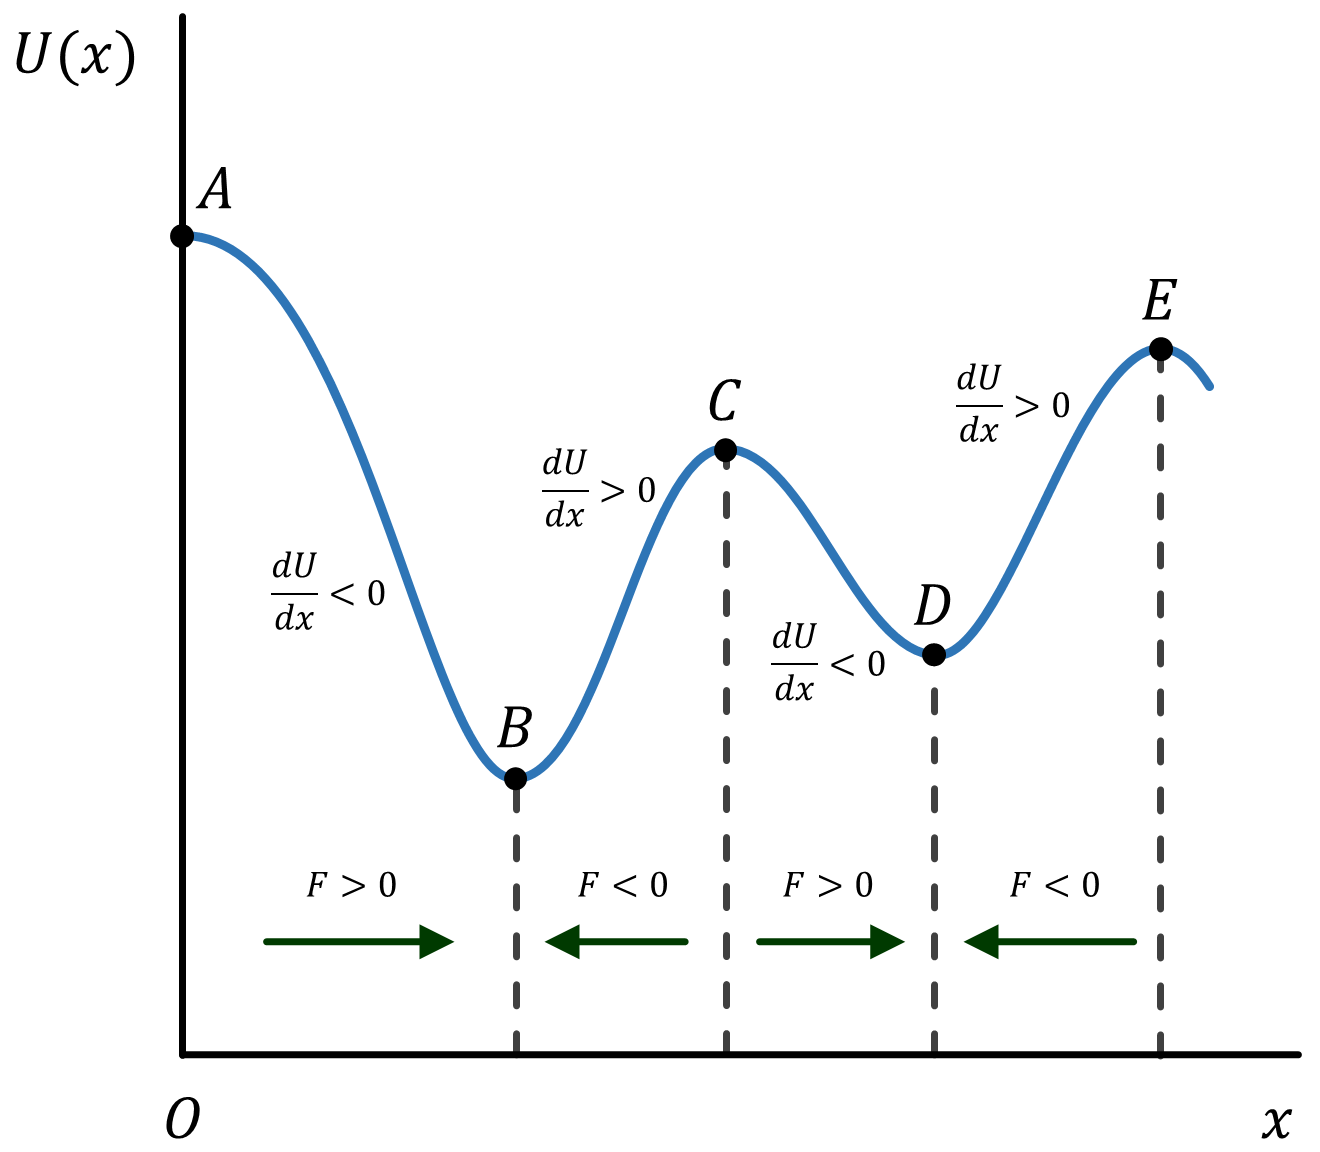
\includegraphics[width=0.48\textwidth]{figures/fig_potential-energy-curve.png}
	\end{wrapfigure}
	In a conservative force field, the potential energy $U$ of a particle is a function of its position in space. A plot showing the variation of potential energy $U$ of a particle with its position (e.g. along the $x$-axis) is known as a \emph{potential energy curve}. This curve provides crucial information about the motion, forces and stability of the particle without requiring the complete solution of its equations of motion.
	
	For one-dimensional motion along the $x$-axis, a conservative force $F$ is obtained from the potential energy function $U(x)$ by the relation:
	\resetwrappadding
	\begin{align*}
		F=-\dv{U}{x}
	\end{align*}
	Thus, the force acting on a particle at any point is equal to the negative slope of the potential energy curve at that point.	
	\begin{itemize}
		\item \emph{Positive slope} (${\text{d}U}/{\text{d}x}>0$): In regions, such as $BC$ and $DE$, where $U$ increases as $x$ increases, the slope $\dv{U}{x}$ is positive. Consequently, the force $F$ is negative, i.e. directed towards the left or in the direction of decreasing $x$.
		
		\item \emph{Negative slope} (${\text{d}U}/{\text{d}x}<0$): In regions, such as $AB$ and $CD$, where $U$ decreases as $x$ increases, the slope $\dv{U}{x}$ is positive. Consequently, the force $F$ is positive, i.e. directed towards the right or in the direction of increasing $x$.
	\end{itemize}
	In either case, the force acting on the particle always tends to move it towards a region of lower potential energy.
	
	\subsection{Concept of equilibrium}
		A particle is said to be in a position of equilibrium when the net force acting on it is zero, i.e.
		\begin{align*}
			\vb{F}_\text{net}=\vb{0}
		\end{align*}
		
		Let us consider a conservative force $F$ acting along the $x$-axis. Then we have
		\begin{align*}
			F=-\dv{U}{x}
		\end{align*}
		If a particle under the influence of the force $F$ is in equilibrium at some point $x_0$, then we have
		\begin{align*}
			F(x_0)&=0 \\
			\implies\left.\dv{U}{x}\right|_{x=x_0}&=0
		\end{align*}
		On a potential energy curve $U(x)$, the slope at the point of equilibrium $x_0$ is zero. Hence, it could either be either on a \emph{local maxima} or on a \emph{local minima} or on a \emph{flat horizontal region}.
		
	\subsection{Types of equilibria}
		The points of equilibria are broadly classified into three types based on how the system responds to a small displacement from the equilibrium position.
		\begin{figure}[h!]
			\centering
			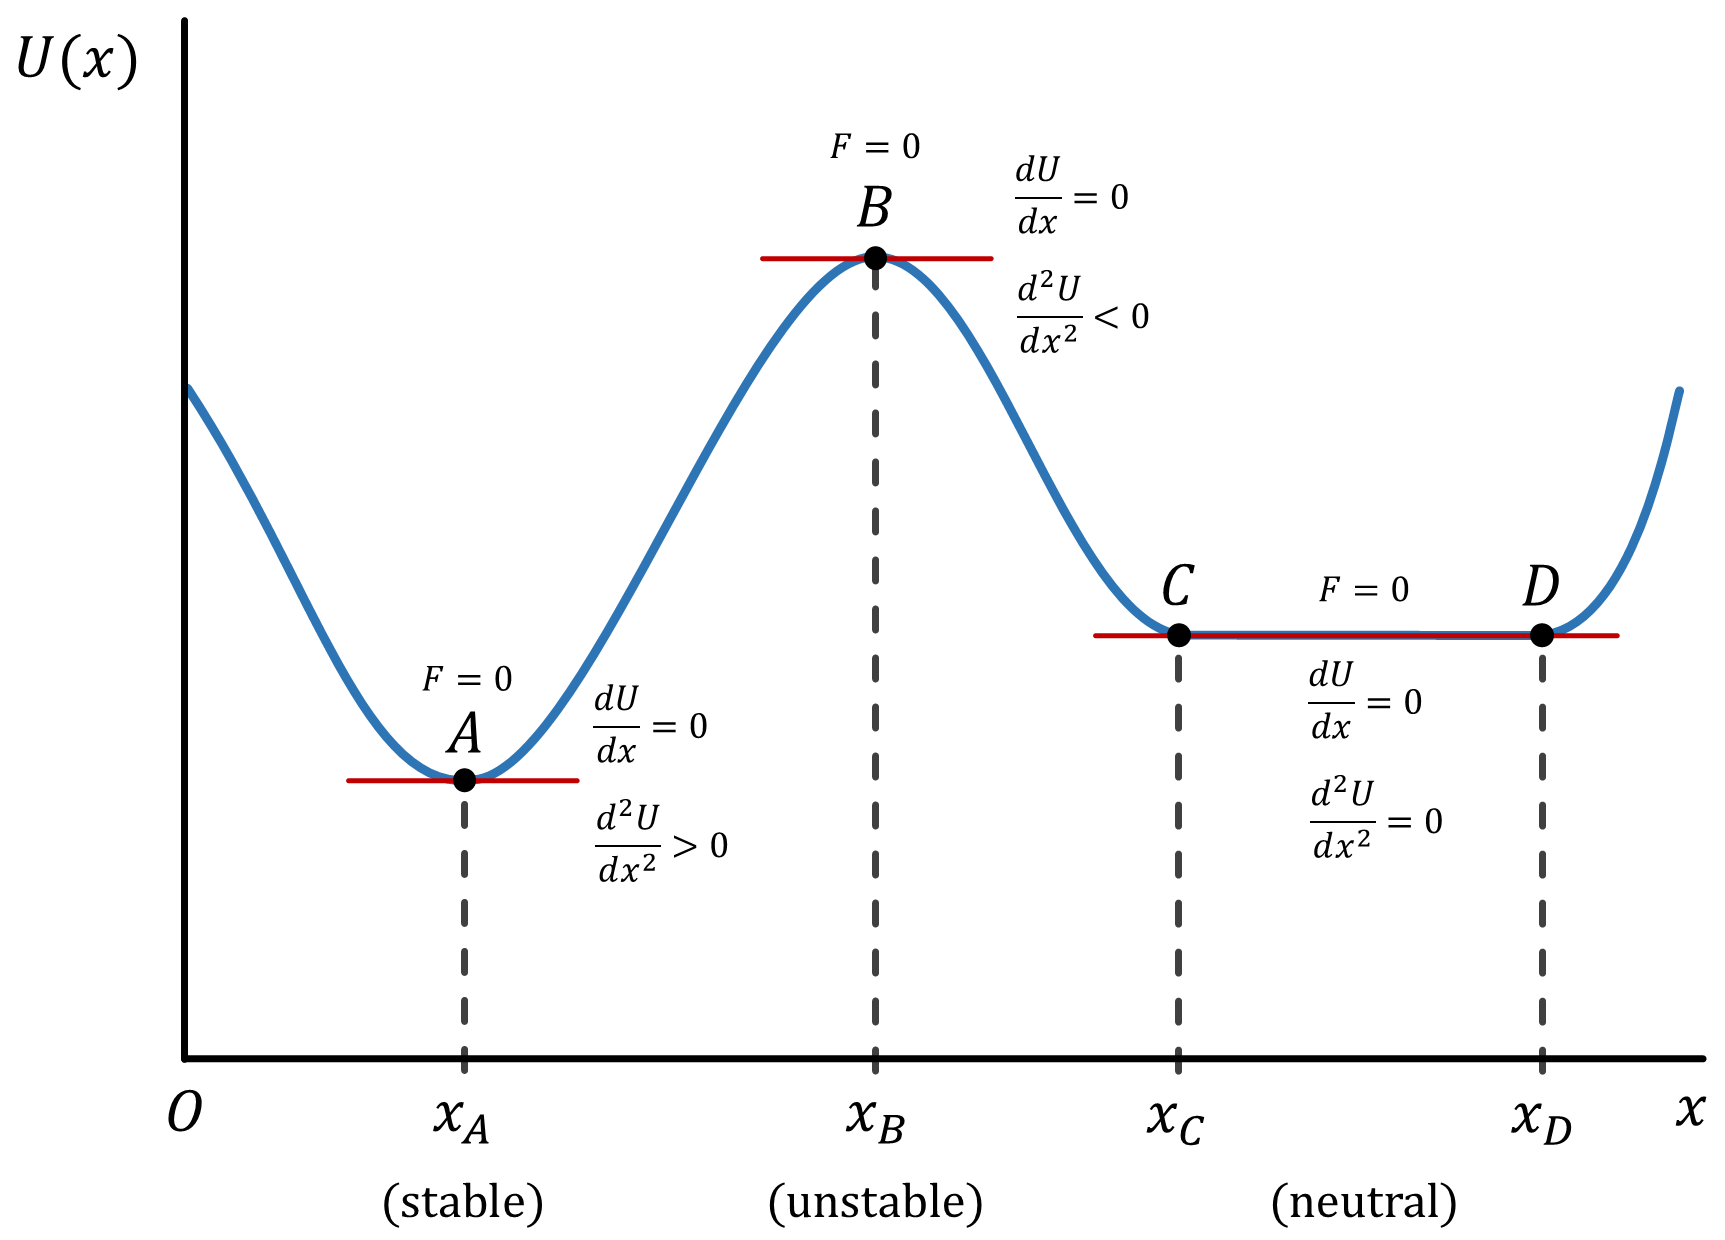
\includegraphics[width=0.7\textwidth]{figures/fig_equilibrium-types.png}
		\end{figure}
		\begin{enumerate}
			\item \textbf{Stable equilibrium:}
				\begin{itemize}
					\item If a particle, which is at a point of stable equilibrium, is slightly displaced in either direction, the resulting force acts in a direction which is opposite to the displacement.
					\item The force acts as a restoring force which pulls the particle back towards its equilibrium position.
					\item Points of stable equilibria occur at local minima, such as point $A$ in the figure above, i.e. $x=x_A$.
					\item At a point of stable equilibrium, we have
					\begin{align*}
						\dv{U}{x}=0\qq{and}\dv[2]{U}{x}>0
					\end{align*}
				\end{itemize}
			
			\item \textbf{Unstable equilibrium:}
				\begin{itemize}
					\item If a particle, which is at a point of unstable equilibrium, is slightly displaced in either direction, the resulting force acts in a direction which is along the displacement.
					\item The force pushes the particle further away from its equilibrium position.
					\item Points of unstable equilibria occur at local maxima, such as point $B$ in the figure above, i.e. $x=x_B$.
					\item At a point of unstable equilibrium, we have
					\begin{align*}
						\dv{U}{x}=0\qq{and}\dv[2]{U}{x}<0
					\end{align*}
				\end{itemize}
			
			\item \textbf{Neutral equilibrium:}
				\begin{itemize}
					\item If a particle, which is at a point of neutral equilibrium, is slightly displaced in either direction, it remains at rest in its new position without tending either to return to its initial position or to move further away.
					\item The force remains zero over the entire region of neutral equilbrium..
					\item Points of neutral equilibria occur over flat horizontal regions, such as the region between points $C$ and $D$ in the figure above, i.e. $x_C<x<x_D$.
					\item At a point of neutral equilibrium, we have
					\begin{align*}
						\dv{U}{x}=0\qq{and}\dv[2]{U}{x}=0
					\end{align*}
				\end{itemize}
		\end{enumerate}